 %\renewcommand{\bottomfraction}{.7}
 %\renewcommand{\textfraction}{.15}
 %\renewcommand{\floatpagefraction}{.66}
 %\renewcommand{\dbltopfraction}{.66}
 %\renewcommand{\dblfloatpagefraction}{.66}
 %\setcounter{topnumber}{9}
 %\setcounter{bottomnumber}{9}
 %\setcounter{totalnumber}{20}
 %\setcounter{dbltopnumber}{9}

 
\newcommand{\makeBasicPlottingFig}{%
\begin{figure*}[tbh]
 \centering
% \includegraphics[width=\linewidth]{basicPlotting}
 \includegraphics[width=1.0\textwidth]{figures/basicPlotting.pdf}
 \caption{A selection of basic plots from PyQtGraph's suite of examples.}
 \label{fig:basicPlotting}
\end{figure*}}

\newcommand{\makePtreeExFig}{%
\begin{figure}[!htbp]
\centering
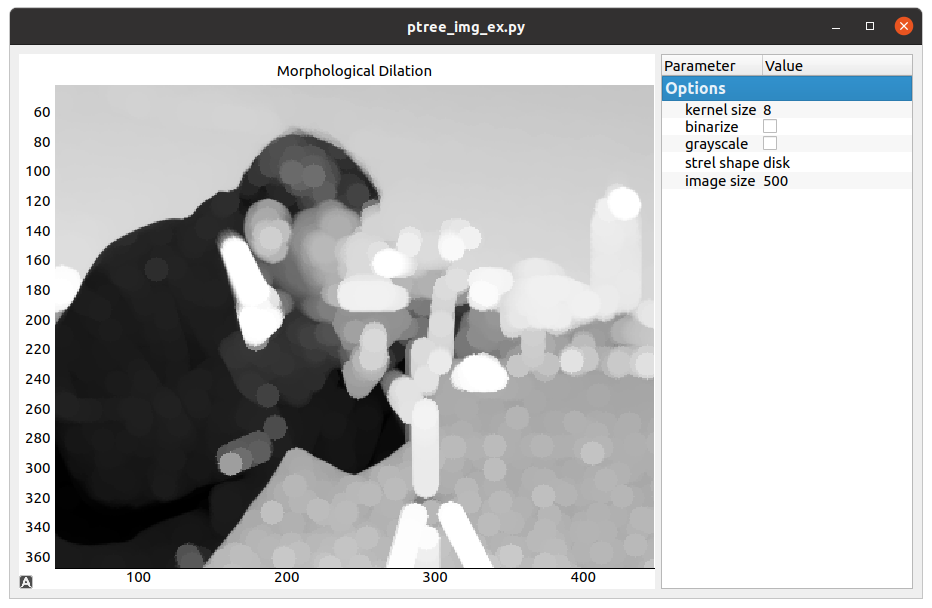
\includegraphics[width=\columnwidth]{figures/pg_ptree_ex.png}
\caption{Sample use of parameter trees for user interaction, where various image processing parameters can be quickly updated. The displayed image reflects these changes in real-time.}
 \label{fig:ptreeEx}
\end{figure}}

\newcommand{\makeNeuralNetFig}{%
\begin{figure*}
\centering
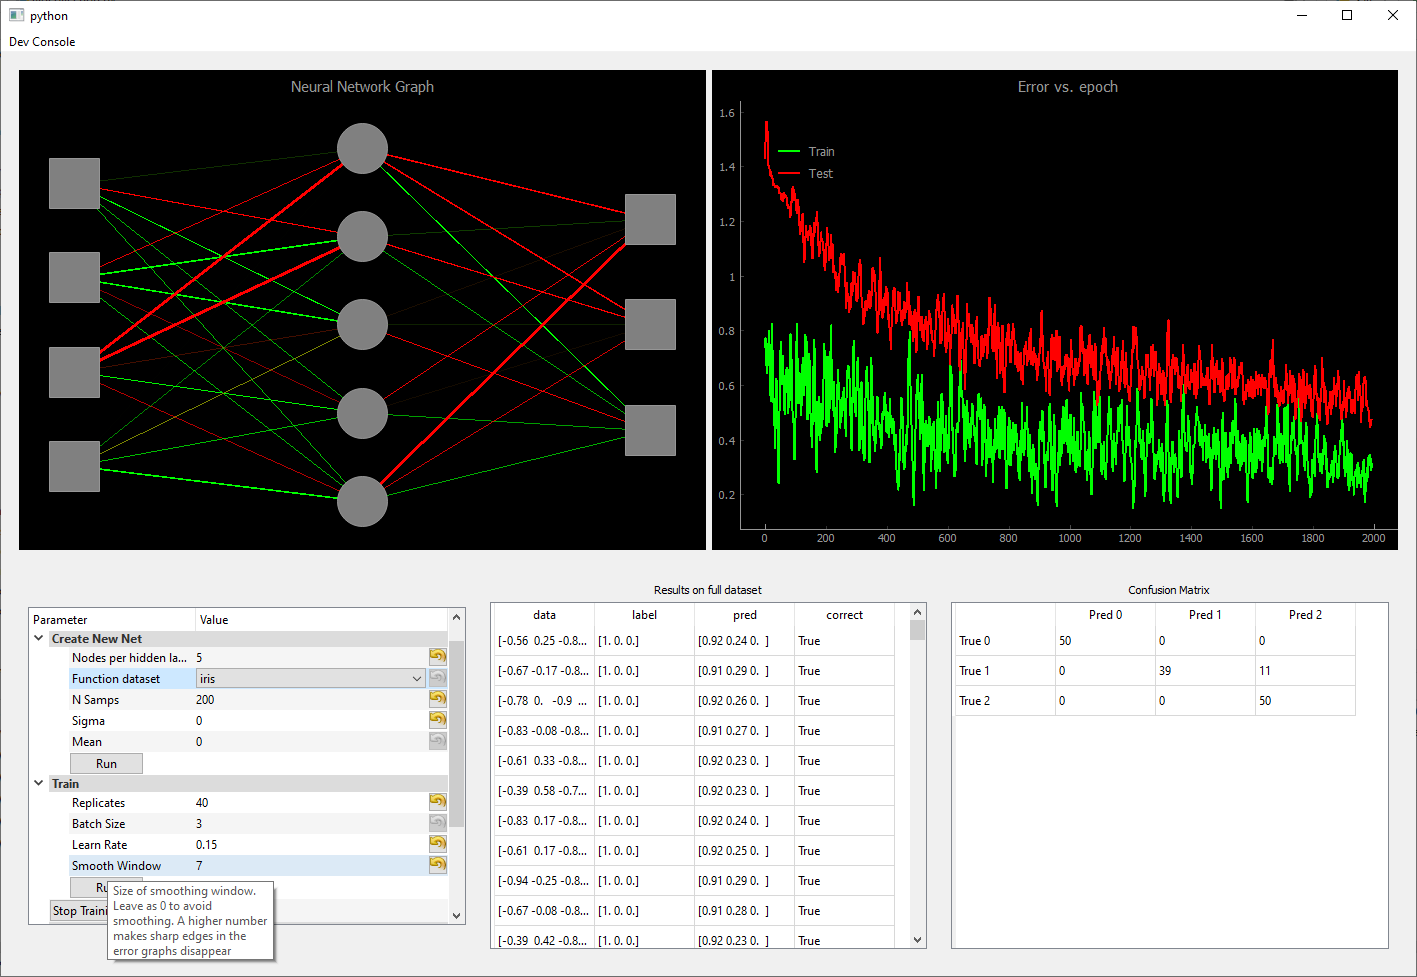
\includegraphics[width=0.8\textwidth]{figures/neuralNetFig.png}
\caption{Application demonstrating how parameter trees, real-time plotting updates, signal hooks, and more can facilitate rapid prototyping and impacts of architectural changes.}
 \label{fig:neuralNetFig}
\end{figure*}}

\newcommand{\makeLineBenchmarkFig}{%
\begin{figure}[!b]
\centering
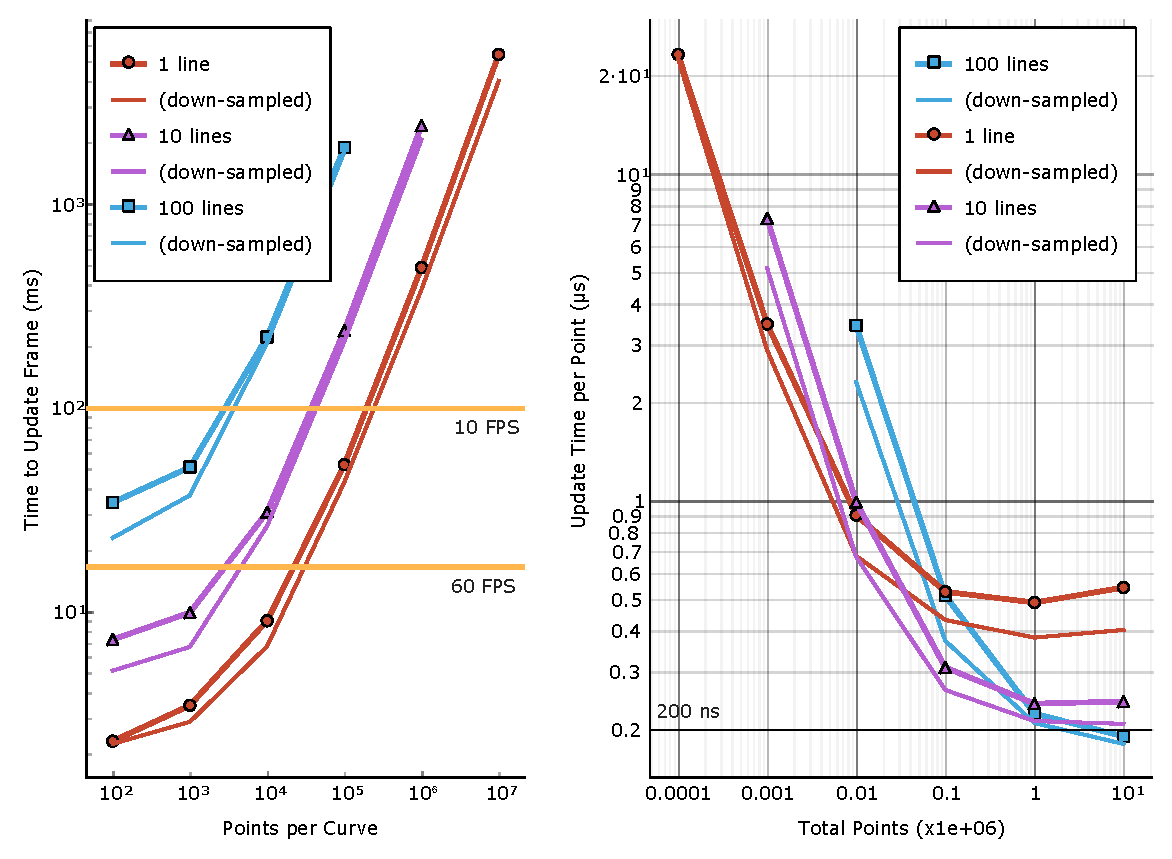
\includegraphics[width=\columnwidth]{figures/lineBenchmark.pdf}
\caption{Line speed benchmark. The time to render 1, 10 or 100 lines of data is shown for varying numbers of points per line. All data was created using an AMD 5900x Ryzen 9 CPU. Left: Time per update over points per curve. The thresholds for achieving 10 and 60 frames/s are shown by horizontal lines. Right: Update time per point, plotted over the total number of points. For more than 100,000 points, the line-plotting time becomes dominant, and the results converge to 200\,ns per point for both 10 and 100 curves, while plotting all points as a single curve increases the time to 500--600\,ns per point.}
 \label{fig:lineSpeed}
\end{figure}
}
 %13-inch 
 
\newcommand{\makeMatplotlibComparison}{%
\begin{figure}[bth]
\centering
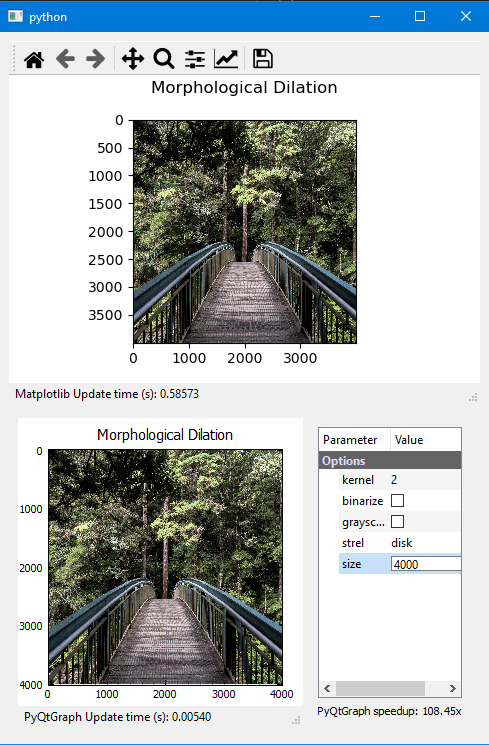
\includegraphics[width=0.9\columnwidth]{figures/pg-mpl-comparison_no_interpolation.png}
\caption{Performance test with PyQtGraph and Matplotlib widgets embedded in a Qt5 application. Over a wide range of image sizes, PyQtGraph completes drawing approximately 75--150 times faster, taking only 5.4\,ms in this example of a 4000\texttimes4000 image. The test is performed without GPU acceleration in a Microsoft Windows environment, and both libraries are set to sub-sample without interpolation. Free-to-use test images are provided by the \href{https://unsplash.com/}{``Unsplash''} service.} 
\label{fig:mpl}
\end{figure}
}

 \newcommand{\makeARBBenchmarkFig}{
 \begin{figure}[tbh]
 \centering
 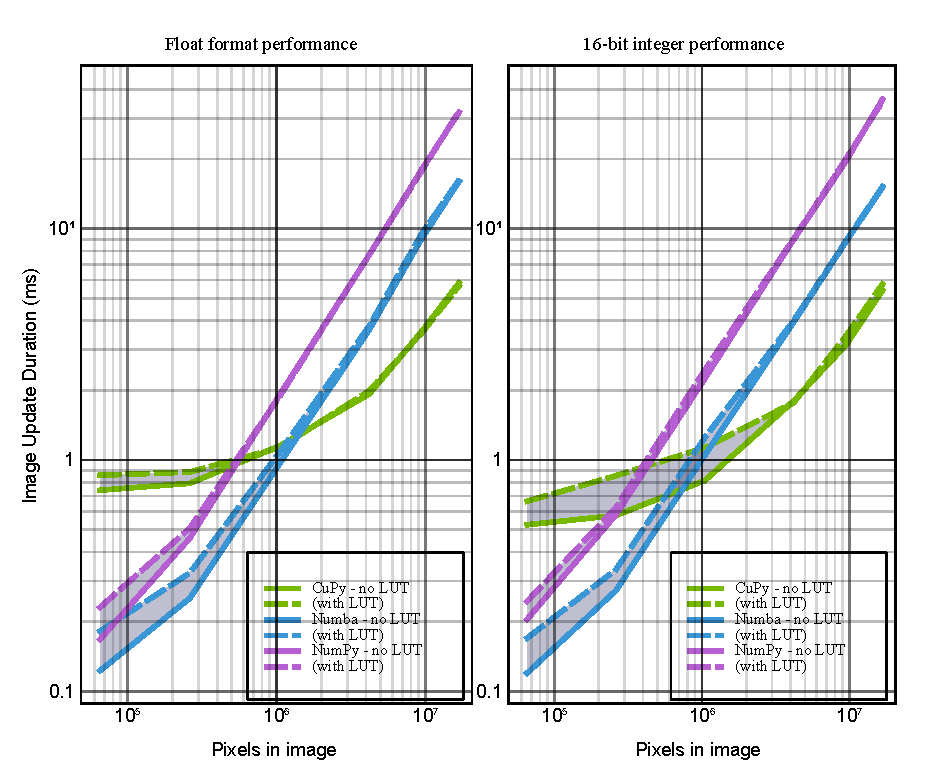
\includegraphics[width=\columnwidth]{figures/makeARGBBenchmark.pdf}
 \caption{Image speed benchmark. The time to update an image frame is shown for different data formats. Left: Using optimized NumPy processing (purple lines), the drawing time is log-scale linear with the number of pixels over a wide range. GPU accelerated CUDA processing using CuPy (green lines) describe a more complex relationship with image size. The need to copy data to and from the GPU creates additional overhead, but as image size grows, the faster processing speed becomes sufficient to compensate for that overhead. The choice of various extra processing tasks like LUTs (dashed lines) show the same basic trends. Alternatively, PyQtGraph's image rendering pipeline can be accelerated in Numba is available on the system.  Benchmarks with Numba (blue lines) can be seen as have performance between that of CuPy and NumPy only. Right: For input data in uint16 format, CUDA processing is particularly advantageous and can provide an almost four-fold reduction in drawing time. Benchmarks were performed on an AMD 5900x Ryzen 9 CPU and an NVIDIA RTX 3080 discrete GPU.}
 \label{fig:makeARGB}
 \end{figure}
 }
 
\newcommand{\makeMonitoringFig}{%
\begin{figure}[!htbp]
\centering
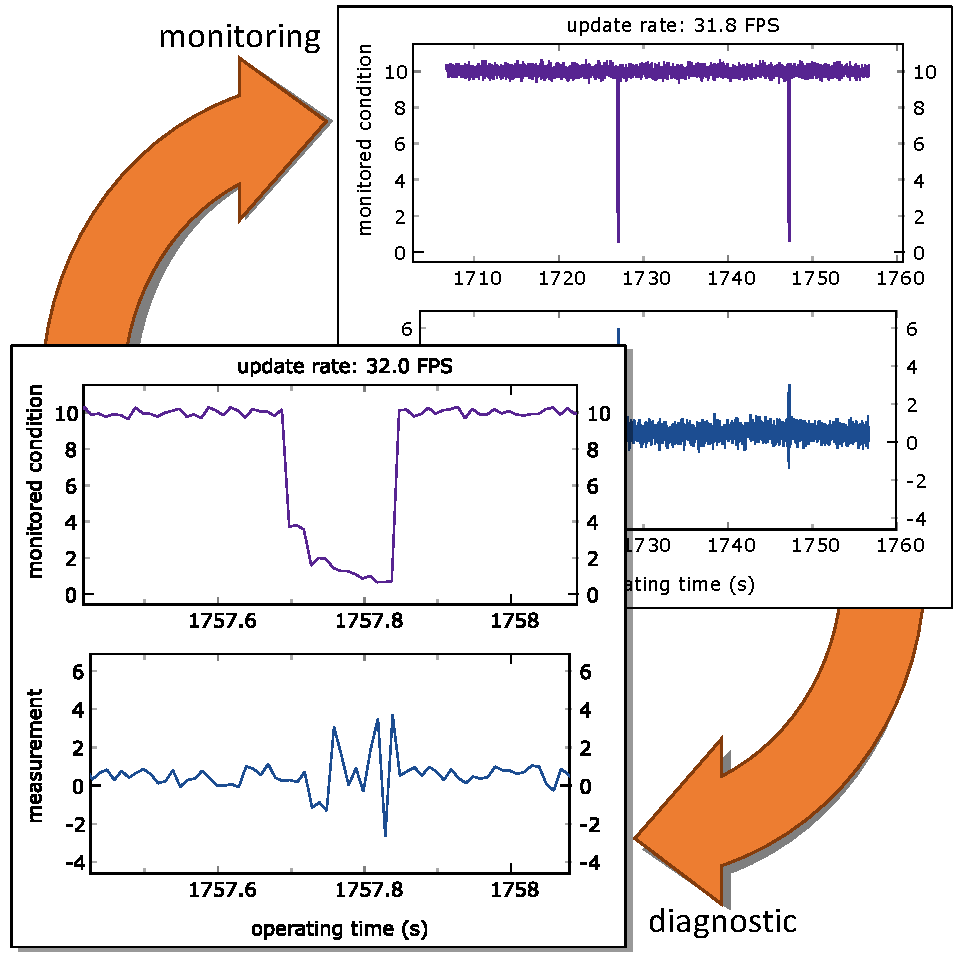
\includegraphics[width=\columnwidth]{figures/monitoring_example_vector.pdf}
\caption{Monitoring and diagnostic of a (simulated) experiment with intermittent failures. Incoming data at 100 samples/s for two measurement channels is recorded into a rolling 5,000 point buffer and continuously displayed at 30 frames/s. When a failure is observed, it can quickly be brought into focus with simple mouse interactions (click-and-drag and mousewheel zoom) for inspection, or to record accurate time stamps. Afterwards, a single click returns the view to automatic scaling without loss of any incoming data.}
 \label{fig:monitoring}
\end{figure}
}




\subsection{Introduction \label{introduction}}

The benefits of interactive exploration of scientific data were recognized as soon as computer systems gained graphical displays. While early implementations like the PRIM-9 system\cite{prim9} of the Stanford Linear Accelerator Center were only available to large installations, more affordable microcomputers soon found their place in smaller laboratories also\cite{Byrd79}\cite{Reed80}, controlling experiments and recording data.

Software packages designed to acquire and process this data soon appeared, with MATLAB\cite{matlab} and LabView\cite{labview} both implementing graphical representation of data from their very first versions. The latter was designed to enable data acquisition, processing and visualization all in the framework of a single program. This approach remains common in fields like statistics where the tools for interaction with data are reasonably well-defined. In other areas, the advent of high-level programming languages like Java and Python has enabled researchers to create the tools for their specific needs with reasonable time investment. This is facilitated by a continuously growing open-source infrastructure that provides resources addressing anything from mathematical methods\cite{numpy2020} to full-scale laboratory data infrastructure\cite{Johnson2015, Koerner2019}.

With less need to recreate existing solutions, it becomes feasible to implement software aiming to reduce turn-around times of iterated experiments: A traditional view of the scientific method envisions a sequence of detailed experiment design, pain-staking note-taking, followed by an exhaustive evaluation resulting in a revised experiment. However, when experiments can be optimized over a wide parameter space, the evaluation quickly becomes the dominant factor. Even for established experimental parameters, external factors such as degraded performance of equipment result in a significant loss of time if they are discovered only in subsequent evaluation.

The solution is to provide immediate feedback to the researcher throughout the experiments, and data visualization has long proven its effectiveness in this regard [Friendly2008]. A challenge lies in providing tools for a detailed inspection of interesting data while new information continues to arrive at rates that for extreme cases are counted in Gb/s even after preselection\cite{LHC}. These tools also need to provide the flexibility to handle data that falls outside the range expected in design, as this is the most likely to indicate failures or to provide the sought-after discovery.

Here we present a visualization library created with these goals in mind. Although written in Python to allow for easy expansion, a close integration with the cross-platform Qt UI framework\cite{Qt} it provides the capability to interactively handle datasets of hundreds of thousands of points, or live representation of high-resolution camera data.

\makeBasicPlottingFig

\section{Approach}
\subsection{Python}
The Python programming language enjoys a large popularity in scientific research due ease of entry and a robust standard library combined with access to very comprehensive numerical computing packages. This makes Python an attractive alternative to established computational tools such as MATLAB\cite{matlab} and Mathematica. %[mathematica].  

The set of most commonly used scientific computing tools in Python are commonly referred to as the SciPy stack. % I think this is still true :)
This refers to SciPy, NumPy, and a variety of other libraries that use the NumPy \texttt{ndarray} data structure as a container for vectorized operations. The \texttt{ndarray} gives developers a high level API to low-level operations with excellent performance. This API allows NumPy and SciPy to provide a wide variety of standard numerical computing operations, all of which are very efficient and help overcome the performance penalty of working with Python as a cross-platform, interpreted, dynamically typed language.

\subsection{Qt}
The Qt framework is a GUI platform written in C++ that allows the creation of cross-platform applications with a single shared code-base. Comprehensive Python bindings (PyQt) expose the complete Qt API. Here, the specific section of interest is the \texttt{GraphicsView} framework, which provides a surface for managing and interacting with a large number of custom-made 2D graphical items, with support for zooming and rotation\cite{QtGraphicsView}. PyQtGraph is built on this foundation to extend the SciPy stack with performant cross-platform visualization.


\subsection{Implementation}
\texttt{GraphicsView} renders line segments in a freely scaled coordinate system through \texttt{QPainterPath} objects. The rendering performance of PyQtGraph results from optimized code to create such paths directly from NumPy ndarrays describing sets of $x$ and $y$ coordinates. The core function \texttt{arrayToQPath} uses NumPy's structured array functionality to efficiently create a binary compatible structure that can serve as an input stream to a \texttt{QPainterPath} item (see Appendix \autoref{app_arrayToQPath}). This \texttt{QPainterPath} is then drawn to the screen by the Graphics View framework.

\section{Capabilities}

All 2d line rendering functions that handle large quantities of data are implemented on top of the \texttt{arrayToQPath} conversion. These cover all common plotting requirements. \autoref{fig:basicPlotting} shows a demonstration from the suite of examples. All graphs included in this paper were generated using PyQtGraph's interactive export functions, which can store both bitmaps and vector formats, or provide access to the raw plotted data.

\subsection{Plot Types}

PyQtGraph shows all plots within a \texttt{PlotItem} object consisting of a \texttt{ViewBox} equipped with a set of axes. This allows dynamic pan and zoom through the transforms of Qt's \texttt{GraphicsView}, with no need to regenerate the \texttt{QPainterPath} objects. Individual elements of the plot are represented by graphics items that share the same coordinate systems and shown in any combination and drawing order. 

PyQtGraph represents line plots as \texttt{PlotCurveItem} objects and offers typical functionality such as color, width and dashing. "Shadow pen" lines can be underlaid for additional contrast. 

Scatter plot items are assigned a default shape, color and size per data set, but each point can also have a unique attributes. Shapes are pre-rendered and cached to optimize performance when the underlying dataset is updated. Depending on the application, symbols can be set to scale with the view or maintain constant size.  Functionality is included for items in scatter plots to recognize mouse hover events.

%An error bar plot is provided that handles $x$, $y$ coordinates, height, width, and lengths in any direction for lines representing errors.  
Plots can be extended by both horizontal and vertical error bars and annotated by text labels. Built in routines can also transform the plotted data to provide logarithmic scaling, Fourier transforms, and to show the gradient $dy/dt$ directly over $t$ or as a phase map over $y$.

Bar graphs and images also make use of this framework and can be added to the same PlotItem, although they are more commonly used separately. Users can also create \texttt{QPainterPath} objects to add their own graphical elements using the well documented methods of the Qt Graphics View framework. PyQtGraph's suite of examples\cite{pg_examples} illustrates this with some demonstrations.


\subsubsection{Performance}

We evaluated the plotting performance for line plots of randomly generated datasets of different length. \autoref{fig:lineSpeed} shows the time taken from setting new data to the completion of the drawing process for 1 to 100 separate curves ranging from 100 to 10 million points. We find that even on common hardware, a curve with 10,000 points can be drawn in less than 10\,ms, and an update rate of 60\,Hz can be maintained up to approximately 30,000 points. Adding more curves introduces additional overhead, such that the same number of 10,000 points, plotted over 100 curves of 100 points each, increases the update time to just below 40\,ms. Nevertheless, the number of points in each of the 100 curves can be increased to close to 3,000 before the update rate falls below 10 frames per second (FPS). At this point, the majority of time is spent processing line segments, and their distribution across different numbers of curves is of secondary importance: A single curve allows for 200,000 points to be displayed at 10 FPS. 

Plotting the results as the update time divided by the overall number of data points further illustrates this. As the total number of points approaches 100,000, where the more or less fixed overhead of the Qt drawing process is no longer significant, the update times converges to approximately 200\,ns per point drawn for both 10 curves and 100 curves. We attribute the increased update time for a single curve to the larger set of data that needs to be handled simultaneously, which may lead to caching issues.

Although the detailed result will vary with platform, system, and data, we consider these results to provide a good reference for the performance that can be expected from PyQtGraph.

\makeLineBenchmarkFig

\subsection{Images and Regions of Interest}

PyQtGraph also provides the means to display images and other multi-dimensional data. Handling streams of such data, as in live video, is similarly enabled by efficient NumPy methods that convert the input data into a binary representation that can be used directly by the Qt framework. Various analysis and processing tools interact with the image arrays, for example regions of interest (ROIs), look-up tables (LUT) for color-mapped display, or histograms.

\subsubsection{Image Views}

\makeARBBenchmarkFig

\makeMatplotlibComparison

The principal object in displaying images, \texttt{ImageItem}, accepts 2-dimensional (interpreted as grayscale) or 3-dimensional (either color or color and alpha) data of any numeric type. Stored in NumPy arrays, this data can be pre-processed efficiently using any available functions in the SciPy stack. Subtracting a background, for instance, is simply a matter of subtracting the reference frame. This input is then processed by \texttt{ImageItem} and converted into Qt's \texttt{QImage} format for rapid display. A range of colormaps are provided to enhance detail perception, and can be altered interactively in levels and colors through a \texttt{HistogramLUTItem}.

\subsubsection{ROIs}

A common image analysis task is to define a ROI in a larger original image. This is supported by multiple interactive objects (\texttt{LineROI}, \texttt{CircleROI}, \texttt{PolygonROI}, and others), which provide NumPy slice objects that reference the selected region within the image array. Once extracted, the relevant data can then be further processed. Magnification, live plotting, FFTs and custom analysis are all simple to implement. Multiple ROIs can be bound together in groups to provide background correction or region comparisons both within a single image stream or across many. These ROI objects remain interactive while attached to the image, so that resizing, moving and rotating a ROI can prompt immediate updates of all subsequent plotting and analysis interfaces.

\subsubsection{Performance}

Numerous factors play into the final performance of a video stream. Data type conversions, LUTs, scaling, and any custom pre-processing all need to occur for each frame, and the computational effort typically scales with image size. A minimum of 20 FPS is generally required for a usable interactive video stream, although 60 FPS is preferred in many applications. In some cases, data can be directly passed to the built-in methods of Qt's \texttt{QImage}. Otherwise \texttt{ImageItem} relies on the core function \texttt{makeARGB} to efficiently convert data types, order data properly, rescale levels and apply a LUT if desired (see \autoref{app_makeARGB}). When integrated as a widget in a Qt application (\autoref{fig:mpl}), we typically find \texttt{ImageItem} to display an image 75--150 times faster than the \texttt{FigureCanvas} provided by Matplotlib, a plotting library that emphasizes graphical quality over speed.

Some share of the image processing is by necessity done in the primary event thread of the Qt application, as that thread requires full access to the data to be displayed. Other calculations can be moved to other threads to improve performance and maintain the responsiveness of the UI. For example, larger images can be down-sampled before handing them to the main thread for display. This multi-threading consideration extends throughout the application, and any excessive use of the event thread will impact image display performance.

\label{sec:cuda}
To further accelerate the handling of large datasets, PyQtGraph can make use of a GPU substrate in one of two ways: \texttt{GLImageItem} or CuPy. \texttt{GLImageItem}, while limited in its interactivity, employs OpenGL for rendering. The CuPy library, a drop-in replacement for NumPy, moves array processing tasks to a CUDA-enabled GPU. This is not beneficial in all applications, since the cost of copying the image data between system memory and the GPU needs to be amortized by a sufficient number of calculations. In the context of image processing, we find that CuPy provides an advantage for images with several hundred thousands of pixels (\autoref{fig:makeARGB}), depending on target hardware.

\subsection{Interactivity}
\subsubsection{Event Driven GUI}
The Qt framework is event driven, which allows PyQtGraph to provide seamless mouse interaction. This also enables users to develop their own desired behavior in response to mouse move, hover, leave, enter, double-click, zoom, or drag events. Almost every aspect of PyQtGraph interacts with the Qt events, or provides its own in response to e.g. axis adjustments or changes to a selected region. This interactivity is a core component of the Qt framework, and adding such behavior to a plot in PyQtGraph is no more complicated than generating the plot in the first place.

\subsubsection{Responsiveness at scale}

Recognizing zoom events enables resolution-aware down-sampling of the plotted data. Multiple available methods provide different trade-offs of accuracy against performance, and include a "peak" display that precisely captures the minima and maxima of the data, a "mean" over the down-sampled interval, and a fast "sub-sample" that displays only 1 in N data points. Zooming into the view automatically reveals more detail of the dataset.

\subsubsection{Parameter Trees}\label{sec:paramtrees}
% \color{DarkOrchid}
Another common requirement for user interaction is a a mechanism to interact with for configuration settings or algorithm parameters. PyQtGraph provides this capability through the \texttt{ParameterTree} object. This takes a simple Python dictionary describing the parameters and leverages existing Qt widgets for editing of text, numeric, list-like, and custom data types. Parameters can be grouped, linked, and dynamically instantiated or removed. Callbacks for user actions or value changes allow results to be recalculated, for experimental equipment to be adjusted immediately, or to implement any other required response. The parameter trees are capable of saving and loading their states hierarchically, to easily create persistent configuration files. Since the access to parameters mimics a Python dictionary, they can function as a drop-in replacement for programmatically adjusted settings that are already implemented as such.

% \color{brown}
% While automated interaction through mouse and keyboard events are critical for seamless user interaction, a mechanism for injecting custom algorithm parameters, configuration settings, and more can be equally important. PyQtGraph provides this capability through Parameter Trees, which allow groupings of arbitrary user-settable data. These leverage existing Qt widgets for text, numeric, list-like, and custom data types while providing callback hooks for when values change or a certain action is triggered. Callbacks can be registered to plot updates, alert messages, data loading, and much more.


% Parameters can be grouped, linked, dynamically instantiated / removed, and reordered as needed. They are also capable of saving/loading their states hierarchically, easily allowing users to generate persistent configuration files. Moreover, since the accessor paradigm for Parameters mimics a Python dictionary, they can function as a drop-in replacement for settings that are currently programmatically modified in the same manner.

% Multiple use cases for these Parameter trees are highlighted in \autoref{sec:examples}. Common to each is the minimal amount of boilerplate additions to facilitate integration and simplicity in setup and customization.

\section{Examples}\label{sec:examples}
% everyone, please put a paragraph/section about a tool you use pyqtgraph for

\subsection{Rapid iteration of processing parameters}

\autoref{fig:ptreeEx} shows such a parameter tree in use. In applications such as image processing, immediate feedback for a choice of algorithmic parameters can help to rapidly reduce the exploration space in the search for viable solutions. For instance, it might be difficult to tell the appropriate kernel size for a morphological operation without testing multiple combinations of image types, parameter values, and more. These factors often make fine-tuning a laborious process. Parameter trees assist in creating a tool to integrate the user with the testing space, quickly and without large amounts of boilerplate code. Using callbacks to provide immediate response, workable parameter combinations can be explored, and candidate solutions can be stored to configuration files, both for comparison to alternative approaches and for application to specific data types.
\makePtreeExFig

\subsection{Model Prototyping}
% \color{DarkOrchid}
The supplementary information contains a similar application of PyQtGraph's capabilities to a machine learning model. Here the parameter trees allows tuning aspects of the input data, model structure and output formats. The plotting functions provide live feedback for how these changes affect model accuracy, greatly assisting a rapid prototyping process.
% \autoref{fig:neuralNetFig}.

% \color{brown}
% Machine learning is one domain in which users can tune some aspects of the input data, model structure, and output formats. In these cases, live feedback for how these changes affect application accuracy can greatly assist the rapid prototyping process. PyQtGraph can facilitate such developments by converting such specifications into tunable knobs. In turn, these updates can be reflected at application runtime -- drastically decreasing the `dead space` between development and visualization. Such a use case is demonstrated in \autoref{fig:neuralNetFig}.
% \makeNeuralNetFig

%-----------------------------------------------------
\renewcommand\textfraction{.05}
\begin{table*}[!hbt]
% \inputminted[
% fontsize=\scriptsize, baselinestretch=0.9, frame=lines, framesep=2mm 
% ]{python}{figures/arrayToQPath_condensed.py}
\begin{verbatim}
def arrayToQPath(x, y, connect='all'):
    """Convert an array of x,y coordinats to QPainterPath as efficiently as possible. The *connect* argument
    may be 'all', indicating that each point should be connected to the next; 'pairs', indicating that each
    pair of points should be connected, or an array of int32 values (0 or 1) indicating connections.
    """

    # condensed variant, full code at:
    # https://github.com/pyqtgraph/pyqtgraph/blob/pyqtgraph-0.12.0/pyqtgraph/functions.py#L1558-L1675
    path = QtGui.QPainterPath()
    n = x.shape[0]
    # create empty array, pad with extra space on either end
    # see: https://github.com/qt/qtbase/blob/dev/src/gui/painting/qpainterpath.cpp
    # All values are big endian--pack using struct.pack('>d') or struct.pack('>i')
    arr = np.empty(n+2, dtype=[('c', '>i4'), ('x', '>f8'), ('y', '>f8')])
    # write first two integers
    byteview = arr.view(dtype=np.ubyte)
    byteview[:16] = 0
    byteview.data[16:20] = struct.pack('>i', n)
    arr[1:-1]['x'] = x # Fill array with vertex values
    arr[1:-1]['y'] = y

    # decide which points are connected by lines
    if eq(connect, 'all'):
        arr[1:-1]['c'] = 1
    elif eq(connect, 'pairs'):
        arr[1:-1]['c'][::2] = 0
        arr[1:-1]['c'][1::2] = 1  # connect every 2nd point to every 1st one
    elif eq(connect, 'finite'):
        isfinite = np.isfinite(x) & np.isfinite(y)
        arr[2:]['c'] = isfinite
    elif isinstance(connect, np.ndarray):
        arr[2:-1]['c'] = connect[:-1]
    else:
        raise Exception('connect argument must be "all", "pairs", "finite", or array')
    arr[1]['c'] = 0  # the first vertex has no previous vertex to connect

    byteview.data[-20:-16] = struct.pack('>i', 0)  # cStart
    byteview.data[-16:-12] = struct.pack('>i', 0)  # fillRule (Qt.OddEvenFill)
    
    # create datastream object and stream into path
    path.strn = byteview.data[16:-12]  # make sure data doesn't run away
    buf = QtCore.QByteArray.fromRawData(path.strn)
    ds = QtCore.QDataStream(buf)
    ds >> path
    return path
\end{verbatim}
\caption{PyQtGraph source code for the core \texttt{arrayToQPath} function.}
\label{table:arrayToQPath}
\end{table*}
%-----------------------------------------------------

%-----------------------------------------------------
\begin{table*}[!tbh]
% \inputminted[
% fontsize=\scriptsize, 
% baselinestretch=0.9,
% frame=lines,
% framesep=2mm
% ]{python}{'figures/makeARGB_condensed.py'}
\begin{verbatim}
import cupy as cp
import numpy as np

def makeARGB(data, lut=None, levels=None, scale=None, useRGBA=False, output=None):
    # condensed variant, full code at:
    # https://github.com/pyqtgraph/pyqtgraph/blob/pyqtgraph-0.12.0/pyqtgraph/functions.py#L1102-L1331
    xp = cp.get_array_module(data) if cp else np

    nanMask = None
    if data.dtype.kind == "f" and xp.isnan(data.min()):
        nanMask = xp.isnan(data)
    # Scaling
    if isinstance(levels, xp.ndarray) and levels.ndim == 2: # rescale each channel independently
        newData = xp.empty(data.shape, dtype=int)
        for i in range(data.shape[-1]):
            minVal, maxVal = levels[i]
            if minVal == maxVal:
                maxVal = xp.nextafter(maxVal, 2 * maxVal)
            rng = maxVal - minVal
            rng = 1 if rng == 0 else rng
            newData[..., i] = (data[..., i] - minVal) * (scale / rng)
        data = newData
    else:
        minVal, maxVal = levels
        rng = maxVal - minVal
        data = (data - minVal) * (scale / rng)
    # LUT
    if xp == cp: # cupy.take only supports "wrap" mode
        data = cp.take(lut, cp.clip(data, 0, lut.shape[0] - 1), axis=0)
    else:
        data = np.take(lut, data, axis=0, mode='clip')

    imgData = output
    if useRGBA:
        order = [0, 1, 2, 3]  # array comes out RGBA
    else:
        order = [2, 1, 0, 3]  # channels line up as BGR in the final image.
    # attempt to use library function to copy data into image array
    fastpath_success = try_fastpath_argb(xp, data, imgData, useRGBA)
    if fastpath_success:
        pass
    elif data.ndim == 2:
        for i in range(3):
            imgData[..., i] = data
    elif data.shape[2] == 1:
        for i in range(3):
            imgData[..., i] = data[..., 0]
    else:
        for i in range(0, data.shape[2]):
            imgData[..., i] = data[..., order[i]]
    if data.ndim != 3 or data.shape[2] != 4:
        imgData[..., 3] = 255
    # apply nan-mask through alpha channel
    if nanMask is not None:
        if xp == cp: # Workaround for https://github.com/cupy/cupy/issues/4693
            imgData[nanMask, :, 3] = 0
        else:
            imgData[nanMask, 3] = 0
    return imgData
\end{verbatim}
\caption{PyQtGraph source code for the core \texttt{makeARGB} function. For brevity, edge cases and null checks have been omitted.}
\label{table:makeARGB}
\end{table*}
%-----------------------------------------------------

\subsection{Monitoring of real-time data}
\makeMonitoringFig
Visualization can provide immediate feedback on measurement results and the operational state of the equipment involved. \autoref{fig:monitoring} shows an application of the opportunities provided by PyQtGraph's interactive facilities in this application. For most applications, no data reduction is necessary to maintain smooth display of a sufficiently large buffer, and no additional code is needed to alternate between monitoring of new data and close inspection of specific events.

\subsection{Additional examples}
The supplementary information includes video demonstrations of two additional applications that make heavy use of PyQtGraph functionality to explore spectral data and to visualize volumetric data representing the 3d structure of multilayer circuit boards.

\section{Software development}
The original motivation for pyqtgraph was in data acquisition software, where there is a need to be able to display video and plots with realtime frame rates and interactivity that allows data exploration. Interactivity was highly important; the established \texttt{matplotlib} library already existed and was excellent for visualizing data in a way that tells a particular story. New data, though, doesn't have this story yet. You want to be able to slice it and stretch it and look at it from every possible angle, quickly and easily, so that you can decide what story to tell.

At the time, most acquisition software would have been written in C/C++ for efficiency. However, newer developments meant python interfaces to Qt's C++ logic provided a good mix between speed and ease of use. PyQwt was perfect for this purpose, but went through a long period without a maintainer (presumably at the time, it was a huge burden maintaining and distributing compiled python packages). So pyqtgraph began as a replacement for PyQwt that would be pure-python, and thus easier to develop and distribute. Following that template, it was also to include UI elements that have common use in acquisition/analysis applications, but are missing from Qt (for example, tools for adjusting image contrast, parameter trees, etc.).

PyQtGraph was first released in 2012, under the open source MIT license. It is known to run on systems ranging from the Raspberry Pi to IBM's s390x architecture. Development is coordinated by volunteer maintainers, with additional code provided by occasional contributors. A continuous integration system asserts that the codebase passes a suite of tests for different combinations of Qt bindings, Python versions and operating systems. PyQtGraph has adopted NEP-29\cite{NEP-29} to establish a support timeline for Python and NumPy versions in line with the rest of the Python community and development occurs in close communication with projects such as ACQ4\cite{10.3389/fninf.2014.00003} and Orange3\cite{JMLR:demsar13a} that constitute a large part of the user base.

\section{Outlook}
With a growing number of both maintainers and contributors, PyQtGraph is well positioned to take advantage of technological developments. The support of hardware acceleration in recent versions of NumPy has already been used to add CUDA integration to some time-critical code, but there is still plenty of potential for further improvements to performance and capabilities. Increased use of multi-threaded patterns is a goal in this respect, both throughout the library, and in user code supported by appropriate documentation, examples and API design. The growing maturity of the Numba just-in-time compiler \cite{lam2015numba} for Python code provides additional opportunities for acceleration beyond what NumPy's array operations can provide.


%% if specified like this the section will be committed in review mode
% \acknowledgments{
% The authors wish to thank all prior, present and future contributors to the PyQtGraph project. Their efforts enable all that is presented here.  Furthermore, we would like to thank maintainers and contributors to the NumPy, SciPy and CuPy projects.}

\section{Appendix}

\subsection{Implementation of arrayToQPath}
\label{app_arrayToQPath}
The function \texttt{arrayToQPath} is at the core of PyQtGraph's plotting performance and is included as \autoref{table:arrayToQPath} to demonstrate the approach.

Execution takes two \texttt{ndarray} objects of the same length, representing $x$- and $y$-coordinates for a series of line segments. Interruptions are relatively rare for the main application of fast line plots, and are represented by interspersed Not-a-Number values. The data is reshaped as a NumPy structured array composed of fields $c$, $x$, and $y$, where $c$ indicates if a connecting line to this point should be drawn. A NumPy \texttt{view} of this array in \texttt{ubyte} format provides direct memory access. The raw memory structure, wrapped in a \texttt{QByteArray} object, can then be used to initialize a \texttt{QPainterPath} object from a \texttt{QDataStream}. All data conversion is handled by NumPy methods that operate more efficiently on the underlying data structure than is possible from Python itself.

\subsection{Implementation of makeARGB}
\label{app_makeARGB}

The function \texttt{makeARGB} provides the data conversions used in displaying image data. It is included here as \autoref{table:makeARGB} to show the approach and the integration of CUDA GPU support discussed in \autoref{sec:cuda}.

The segment of memory within a \texttt{QImage} object that will ultimately be displayed on the screen can be accessed and written to as a contiguous, row-major, 3-dimensional NumPy \texttt{ndarray} of unsigned 8-bit integers; i.e. the red, green and blue color values and alpha value of each pixel, one row at a time. With this array as the output target, an incoming image data goes through a number of processing steps. Many of the steps are only conditionally executed, depending on the shape and type of the incoming data, as well as the use of LUTs or rescaling. Some of the respective branches and decision trees have been omitted here for brevity. In a best-case scenario, the incoming data is already in the correct format, and the steps converting data type and element order can then also  be omitted. The CuPy library provides CUDA support by replicating large sections of NumPy functionality, allowing for near-identical code paths. The two if-statements seen here address the lack of a 'clip' mode in CuPy's 'take' function, as well as differing behavior for masks as indices.
